\documentclass[conference]{IEEEtran}
\usepackage{graphicx,booktabs,amsmath,amssymb,multirow,tabularx,array,url,cite}
\usepackage[hidelinks]{hyperref}
\graphicspath{{figures/}}
\title{AKC-Tutor: An Affect- and Knowledge-Aware Conversational AI Framework for Personalized Intelligent Tutoring}
\author{\IEEEauthorblockN{Shiva Nayak Dharavath\IEEEauthorrefmark{1}, Raju Shanmugam\IEEEauthorrefmark{2}}
\IEEEauthorblockA{Department of Computer Science and Engineering\\
Vel Tech Rangarajan Dr. Sagunthala R\&D Institute of Science and Technology\\
Avadi, Chennai, India\\
\IEEEauthorrefmark{1}vtd1556@veltech.edu.in \quad \IEEEauthorrefmark{2}srajuhere@gmail.com\\
ORCID: \IEEEauthorrefmark{1}0009-0003-6756-6789; \IEEEauthorrefmark{2}0000-0002-8613-9518\\
Corresponding author: Shiva Nayak Dharavath}}
\begin{document}
\maketitle
\begin{abstract}
Personalized tutoring needs to adapt explanations to a learner's estimated understanding while responding appropriately to emotional cues. This paper presents AKC-Tutor, a modular framework evaluated through emotion classification, educational interaction prediction, and controlled tutoring-response assessment. On 4,590 held-out single-label GoEmotions examples, RoBERTa achieved 62.79\% accuracy and 48.24\% macro-F1, compared with 56.19\% and 37.36\% for TF--IDF logistic regression. On 57,690 held-out educational interactions from a learner-disjoint split, knowledge-plus-behavioral features attained ROC-AUC 0.8182 versus 0.7841 for knowledge-only features (cluster-bootstrap difference 0.0341, 95\% CI [0.0278, 0.0419]). A separate template-based policy generated 96 responses for 24 researcher-authored scenarios under generic, knowledge-only, emotion-only, and combined conditions. Two evaluator workbooks supplied 192 complete response ratings. The combined condition improved rated affective appropriateness over knowledge-only by 0.458 points on a five-point scale (scenario-paired 95\% CI [0.208, 0.708], Holm-adjusted $p=0.0136$), without a significant improvement in correctness, helpfulness, or knowledge fit. The datasets are not learner-aligned, and neither actual student learning gains nor end-to-end emotion--knowledge personalization are demonstrated.
\end{abstract}
\begin{IEEEkeywords}
Intelligent tutoring systems, affective computing, educational data mining, knowledge tracing, emotion classification, conversational tutoring.
\end{IEEEkeywords}
\section{Introduction}
Intelligent tutoring systems aim to respond to differences in student understanding rather than provide a fixed explanation to every learner. Knowledge tracing predicts learner performance from previous interactions \cite{piech2015}. Recent reviews also describe personalized tutoring as a major application of artificial intelligence in education \cite{wang2024}. Yet prediction accuracy alone does not establish whether a tutor's response is pedagogically appropriate. A student asking for a hint, expressing frustration, or requesting a harder question may require different wording and instructional support.

Affective information presents a complementary but difficult signal. The GoEmotions benchmark provides fine-grained emotion annotations for Reddit comments \cite{demszky2020}. Transformer encoders such as RoBERTa can classify such text \cite{liu2019}, but transferring emotion recognition to real educational dialogue remains an open validation problem. Meanwhile, educational interaction logs typically lack aligned emotion annotations. These constraints motivate a modular evaluation that separates observed evidence from proposed end-to-end capability.

This work makes three contributions. First, it compares a sparse-text baseline with RoBERTa on the same held-out single-label emotion classification task. Second, it quantifies the predictive value of past behavioral-history features alongside knowledge features on learner-disjoint educational records, including a shuffled-behavior control. Third, it evaluates four auditable template-based tutoring variants with two independently supplied rating workbooks and scenario-paired statistical comparisons. The contribution is a controlled component-level investigation, not a deployed learning intervention.

\section{Related Work}
\subsection{Knowledge-Aware Educational Modeling}
Knowledge tracing formalizes the prediction of a learner's subsequent responses from their interaction history. Deep Knowledge Tracing introduced recurrent models for this task \cite{piech2015}. Our educational experiment instead evaluates a reproducible feature-based predictive baseline and tests whether past behavioral information adds predictive value under learner-disjoint splitting. We do not equate historical behavior features with emotion.
\subsection{Text-Based Affect Recognition}
GoEmotions comprises manually labeled English Reddit comments and a taxonomy of 27 emotions plus neutral \cite{demszky2020}. RoBERTa is a robustly optimized pretrained transformer encoder \cite{liu2019}. A model trained on GoEmotions may recognize general linguistic cues, but the source corpus does not establish accuracy for actual student dialogue. Accordingly, our study treats predicted emotions as experimental conditions, not verified psychological states.
\subsection{Conversational Tutoring Evaluation}
Reviews of AI in education identify adaptive tutoring among prominent applications while emphasizing the need for rigorous evaluation \cite{wang2024}. Studies of AI feedback show that apparently suitable responses need not improve learning outcomes \cite{liebenow25}. Our response study isolates instructional and affective conditioning using fixed templates, rather than claiming a generative large language model or measured learner outcomes.

\subsection{Knowledge Tracing and Behavioral History}
Recent knowledge tracing studies represent student--skill relations using heterogeneous interaction graphs \cite{xu23}. Target hierarchies permit finer-grained state estimates \cite{sun24}. Question factors, including difficulty, add contextual information beyond correctness history \cite{zhao23}. Response speed can be modeled as a complementary learning signal \cite{huang24speed}. Temporal and causal enhancements address uneven exposure to concepts \cite{huang24causal}. Graph pretraining seeks more informative representations from sparse interaction histories \cite{zhu24}.

Option-aware mixtures of experts exploit more than binary correctness \cite{huang24moe}. Multiple knowledge relations can be fused into tracing models \cite{duan24}. Hyperbolic embeddings represent relations among tutoring entities \cite{liu24hyper}. Concept maps and unchosen response options may help characterize errors \cite{park24concept}. Long- and short-term knowledge graphs model different time scales \cite{yu25graph}. Progressive models distinguish stages of the learning process \cite{sun24progress}. Spatiotemporal graph models follow changing concept relations \cite{yang24hetero}.

Recent heterogeneous graph tracing combines contrastive views and meta-path contexts \cite{liu26contrast}. Transfer-aware graph representations connect knowledge concepts \cite{yang25mahkt}. Student--question graphs incorporate attempts and hints \cite{xu26sqg}. Coarse--fine-grained models examine the granularity of latent states \cite{luo24}. Learning-state representations model diverse response patterns \cite{wang25states}. Cognitive-situation models link tracing to psychological constructs \cite{wu25cognitive}. Programming-specific graphs show the importance of task context \cite{wu24program}. Information-processing graphs provide an alternative account of sequential performance \cite{xiao26}. These studies motivate our feature ablation; none of their architectures is claimed as an implemented comparator.

\subsection{Educational Affect and Feedback}
A review of automated emotion recognition identifies limited evidence of deployment in authentic learning environments \cite{yu24emotion}. A review of affective computing in online higher education also reports a gap between technical detection and educational application \cite{affect26}. Studies of instructors' emotional expressions distinguish attentional effects from knowledge retention \cite{zhang24video}. Experimental work on LLM-generated feedback reports that its benefits may depend on learners' initial self-assessment \cite{liebenow25}. These findings motivate evaluating response appropriateness separately from measured learning outcomes.

\section{AKC-Tutor Framework}
\begin{figure*}[t]
\centering
\setlength{\fboxsep}{7pt}
\fbox{\begin{minipage}{0.94\textwidth}\centering
\textbf{Input stream A: text emotion cues}\ $\downarrow$ \\ RoBERTa classifier (GoEmotions) $\rightarrow$ predicted affect label \\[4pt]
\textbf{Input stream B: learner interaction history}\ $\downarrow$ \\ Past-only knowledge features $+$ behavioral-history proxies $\rightarrow$ correctness probability \\[4pt]
\rule{0.75\linewidth}{0.3pt}\\[4pt]
\textbf{Controlled scenario interface:} researcher-authored student text + illustrative held-out knowledge probability\\ $\downarrow$ \\ Four policies: generic $\mid$ knowledge-only $\mid$ emotion-only $\mid$ combined \\ $\downarrow$ \\ Auditable template responses $\rightarrow$ blinded 1--5 rubric ratings\\[2pt]
\textit{Dashed conceptual connection: the two datasets are unpaired; no shared real learner state is observed.}
\end{minipage}}
\caption{AKC-Tutor experimental workflow. Emotion classification, educational prediction, and response assessment are separate modules; the scenario interface does not constitute verified learner-level multimodal fusion.}\label{fig:architecture}
\end{figure*}
The architecture contains three modules. The text module maps a statement $x$ to a predicted emotion $\hat e=\arg\max_k p(e_k\mid x)$. The educational module estimates the probability of next-response correctness from past-only features, $\hat p_t=P(y_t=1\mid K_{<t},B_{<t})$, where $K$ denotes knowledge-history features and $B$ denotes behavioral-history proxies. The response module maps a scenario, an illustrative knowledge level, and an optional predicted emotion to a researcher-authored response template.

The response policies differ by available conditioning information. The generic condition ignores knowledge and affect. The knowledge-only condition adapts instructional action to the supplied knowledge state. The emotion-only condition adjusts tone using predicted affect. The combined condition uses knowledge for instructional action and affect for phrasing. Thus, the experiment tests response-level conditioning; it does not demonstrate that emotion changed instructional-action selection.

\section{Experimental Design}
\subsection{Phase I--II: Emotion Classification}
The single-label subset of the official simplified GoEmotions splits contains 36,308 training, 4,548 validation, and 4,590 test records across 28 labels. Multilabel examples are excluded. Phase I uses TF--IDF features with logistic regression; regularization is selected using validation performance, followed by refitting on training plus validation data. Phase II fine-tunes \texttt{FacebookAI/roberta-base} with maximum token length 128, batch size 16, gradient accumulation 2, learning rate $2\times10^{-5}$, weight decay 0.01, and three requested epochs. The checkpoint is selected by validation macro-F1, with a held-out test evaluation. The recorded seed is 42. We report accuracy, macro-F1, weighted-F1, and bootstrap uncertainty.
\subsection{Phase III: Educational Prediction}
The educational interaction file used by the experiment contains 525,534 raw and 446,844 cleaned records, representing 4,151 learners and 110 skills. Learner-disjoint train, validation, and test splits contain 331,474, 57,680, and 57,690 interactions, respectively (2,905, 622, and 624 learners). Features use past interactions only. Five alternatives are compared: knowledge-only, behavioral-proxy-only, knowledge-plus-behavior, shuffled behavioral features, and constant training prevalence. The primary endpoint is test ROC-AUC. A learner-cluster bootstrap (500 replicates) estimates uncertainty in the fusion-minus-knowledge AUC difference. The dataset has no observed affect annotations in this experiment.
\subsection{Phase IV: Response Generation}
Twenty-four researcher-authored scenarios cover linear equations, fractions, and probability. Each scenario yields four responses, totaling 96. The policy is template-based and auditable, not a trained generative tutor. Emotion labels are model predictions; knowledge probabilities are illustrative draws from the Phase III held-out prediction distribution, not probabilities computed from the scenario speaker's own history. Automated conformity checks only verify expected template behavior and cannot establish educational quality.
\begin{figure}[t]\centering
\setlength{\fboxsep}{3pt}\fbox{\begin{minipage}{0.92\columnwidth}\centering\footnotesize
24 researcher-authored scenarios\\[3pt]$\Downarrow$\\[3pt]
\begin{tabular}{cc}\fbox{Generic} & \fbox{Knowledge only}\\[4pt]\fbox{Emotion only} & \fbox{Combined}\end{tabular}\\[4pt]$\Downarrow$\\[3pt]
96 deterministic responses $\rightarrow$ two blinded rating workbooks\\[3pt]
4 criteria $\times$ 2 evaluators; scenario-paired inference
\end{minipage}}
\caption{Phase IV--V controlled response generation and evaluation design.}\label{fig:policy}\end{figure}
\subsection{Phase V: Human Rubric and Inference}
Two submitted evaluator workbooks contain complete ratings for the same 96 response IDs. Each response is scored on correctness, helpfulness, knowledge appropriateness, and affective appropriateness using integers from 1 to 5. Evaluator independence is author-attested rather than externally authenticated. Exact agreement and quadratic-weighted Cohen's $\kappa$ assess consistency. For comparisons, the two ratings are averaged within each scenario and policy; 24 scenario-paired differences compare combined with knowledge-only. Confidence intervals use 30,000 scenario bootstrap resamples; two-sided sign-flip tests use 200,000 Monte Carlo permutations, and Holm adjustment covers four outcomes. These are response-quality ratings, not observed learning gains.

\subsection{Research Questions and Leakage Controls}
The experiments address three questions: (RQ1) whether a pretrained encoder improves fine-grained text emotion classification; (RQ2) whether past behavioral features add predictive information to knowledge history on unseen learners; and (RQ3) whether affect-conditioned phrasing improves rated response suitability compared with knowledge-only tutoring. The answers come from distinct datasets, not a single jointly trained learner model.

The emotion experiments retain a held-out test set. The educational split excludes test learners from training, and history features use past interactions only. The response comparison pairs all four policies within each scenario. Pairing limits between-scenario variation but does not remove biases associated with researcher-written templates or rubric interpretation.

\subsection{Operational Policy Design}
The policy comparison separates \emph{action selection} from \emph{surface realization}. Let $q\in\{L,M,H\}$ be the supplied knowledge band and $e$ the predicted emotion label. The knowledge-conditioned instructional action is $a=g(q)$; in the combined condition, the response is $r=T(a,e)$, where $T$ is a deterministic researcher-written template. For knowledge-only, $r=T(a,\varnothing)$; for emotion-only, $r=T(a_0,e)$ with a fixed generic instructional action $a_0$. This design tests whether affect changes response wording while holding the instructional decision rule explicit.

The experimental design is balanced: $24$ scenarios $\times$ $4$ policies $=96$ responses. Scenarios span fractions, linear equations, and probability. Because the supplied knowledge estimates are illustrative rather than inferred from the scenario speakers, we do not treat the responses as personalized interactions with actual learners. This distinction prevents a circular claim that separate predictive modules were jointly validated.

\subsection{Statistical Estimands}
For a rubric dimension $d$, let $r_{isjd}$ denote the score from evaluator $j$ for scenario $i$ under policy $s$. The scenario-level score is $\bar r_{isd}=\frac{1}{2}\sum_{j=1}^{2}r_{isjd}$. The primary effect is
\begin{equation}
\widehat\Delta_d=\frac{1}{24}\sum_{i=1}^{24}(\bar r_{i,\mathrm{combined},d}-\bar r_{i,\mathrm{knowledge},d}).
\end{equation}
Resampling the $24$ scenario indices preserves the matched comparison and within-scenario dependence. The confidence interval summarizes scenario variability; the sign-flip null assumes exchangeability of paired effect signs. Holm adjustment addresses four prespecified rubric comparisons. Weighted $\kappa$ is computed separately by dimension to account for ordinal distances between evaluator ratings.

\section{Results and Discussion}
\subsection{Emotion Recognition}
\begin{table}[t]\centering\caption{Held-Out Emotion Classification ($n=4590$)}\label{tab:emotion}\begin{tabular}{lccc}\toprule Model & Acc. & Macro-F1 & Wtd.-F1\\\midrule TF--IDF + LR & 0.5619 & 0.3736 & 0.5267\\ RoBERTa & \textbf{0.6279} & \textbf{0.4824} & \textbf{0.6183}\\\bottomrule\end{tabular}\end{table}
RoBERTa increases macro-F1 by 0.1089 absolute points (Table~\ref{tab:emotion}, Fig.~\ref{fig:emotion}). Its recorded bootstrap 95\% macro-F1 interval is [0.4653, 0.4968], compared with [0.3567, 0.3884] for the classical baseline. These intervals describe model performance on the selected Reddit-derived single-label test distribution, not performance on educational dialogue.
\begin{figure}[t]\centering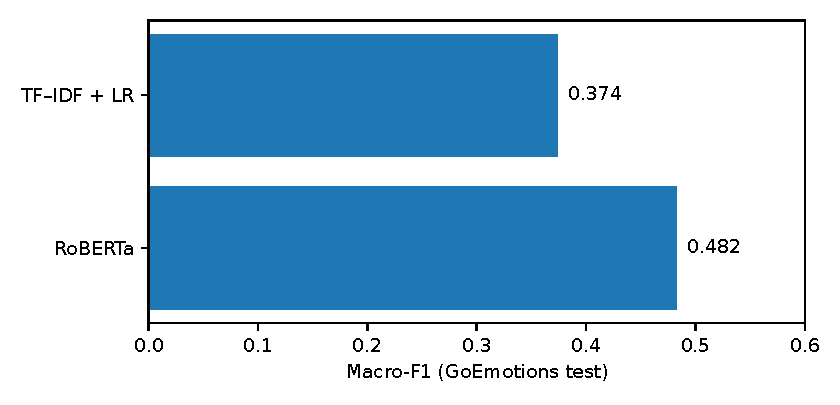
\includegraphics[width=\columnwidth]{phase12_emotion.pdf}\caption{Macro-F1 of the two emotion models on the held-out test set.}\label{fig:emotion}\end{figure}
\subsection{Knowledge and Behavioral-History Prediction}
\begin{table}[t]\centering\caption{Learner-Disjoint Educational Test Performance}\label{tab:knowledge}\begin{tabular}{lccc}\toprule Model & AUC & Acc. & F1\\\midrule Knowledge-only & 0.7841 & 0.7637 & 0.8416\\ Behavioral-only & 0.7810 & 0.7826 & 0.8479\\ \textbf{Knowledge + behavior} & \textbf{0.8182} & \textbf{0.7942} & \textbf{0.8606}\\ Shuffled behavior & 0.7841 & 0.7636 & 0.8415\\ Constant prevalence & 0.5000 & 0.7097 & 0.8302\\\bottomrule\end{tabular}\end{table}
The combined educational predictor attains ROC-AUC 0.8182 (Table~\ref{tab:knowledge}, Fig.~\ref{fig:auc}), improving over knowledge-only by 0.0341 (learner-cluster bootstrap 95\% CI [0.0278, 0.0419]). Shuffling the behavioral features removes this improvement (AUC 0.7841). This supports the predictive value of historical behavioral features, but does not test true emotion--knowledge fusion.
\begin{figure}[t]\centering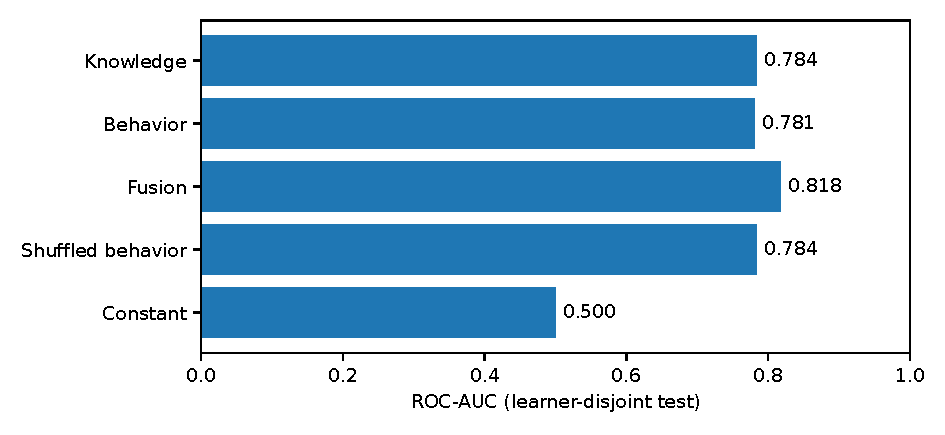
\includegraphics[width=\columnwidth]{phase3_auc.pdf}\caption{Educational prediction ablation on held-out learners.}\label{fig:auc}\end{figure}
\subsection{Controlled Tutoring Responses and Ratings}
\begin{table}[t]\centering\caption{Mean Human Rubric Scores (Two Raters, 1--5)}\label{tab:ratings}\scriptsize\setlength{\tabcolsep}{3pt}\begin{tabular}{lcccc}\toprule Policy & Corr. & Help. & Know. & Affect\\\midrule Generic & 4.083 & 3.167 & 3.354 & 2.792\\ Knowledge-only & \textbf{4.521} & 3.479 & 3.500 & 2.979\\ Emotion-only & 4.188 & 3.458 & \textbf{3.625} & 3.313\\ Combined & \textbf{4.521} & \textbf{3.563} & 3.563 & \textbf{3.438}\\\bottomrule\end{tabular}\end{table}
The combined variant has the highest mean affective-appropriateness rating (3.438), versus 2.979 for knowledge-only (Table~\ref{tab:ratings}, Fig.~\ref{fig:ratings}). It ties knowledge-only on correctness and has a slightly higher mean helpfulness score. Emotion-only has the highest observed knowledge-fit mean, illustrating that combined conditioning is not uniformly best on every metric.
\begin{figure}[t]\centering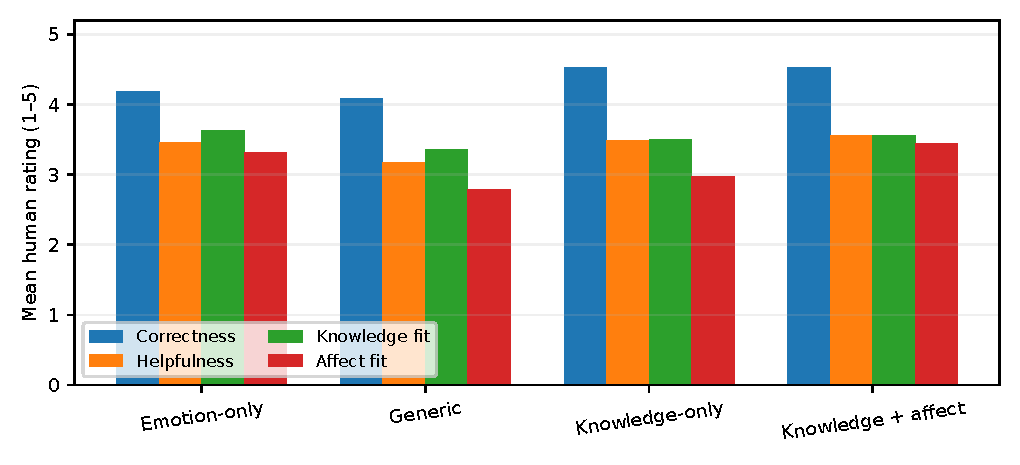
\includegraphics[width=\columnwidth]{phase5_variant_ratings.pdf}\caption{Pooled human ratings by policy and rubric dimension.}\label{fig:ratings}\end{figure}
\begin{table}[t]\centering\caption{Inter-Rater Agreement ($n=96$ Responses)}\label{tab:agreement}\begin{tabular}{lcc}\toprule Criterion & Exact agree. & Weighted $\kappa$\\\midrule Correctness & 82.29\% & 0.768\\ Helpfulness & 44.79\% & 0.638\\ Knowledge fit & 50.00\% & 0.510\\ Affective fit & 71.88\% & 0.609\\\bottomrule\end{tabular}\end{table}
Quadratic-weighted agreement ranges from 0.510 to 0.768 (Table~\ref{tab:agreement}); exact agreement is lower for helpfulness and knowledge fit. The rating scales are ordinal, and agreement is not evidence of learning efficacy.
\begin{table}[t]\centering\caption{Combined Minus Knowledge-Only: 24 Paired Scenarios}\label{tab:paired}\scriptsize\setlength{\tabcolsep}{3pt}\begin{tabular}{lccc}\toprule Criterion & $\Delta$ & Bootstrap 95\% CI & Holm $p$\\\midrule Correctness & 0.000 & [$-0.083$, $0.083$] & 1.000\\ Helpfulness & 0.083 & [$-0.125$, $0.271$] & 1.000\\ Knowledge fit & 0.063 & [$-0.083$, $0.208$] & 1.000\\ Affective fit & \textbf{0.458} & \textbf{[$0.208$, $0.708$]} & \textbf{0.0136}\\\bottomrule\end{tabular}\end{table}
Only affective appropriateness shows a statistically supported difference after adjustment (Table~\ref{tab:paired}, Fig.~\ref{fig:effects}). The observed benefit is consistent with an affect-conditioned phrasing mechanism. It does not establish improved instructional decision-making or student achievement.
\begin{figure}[t]\centering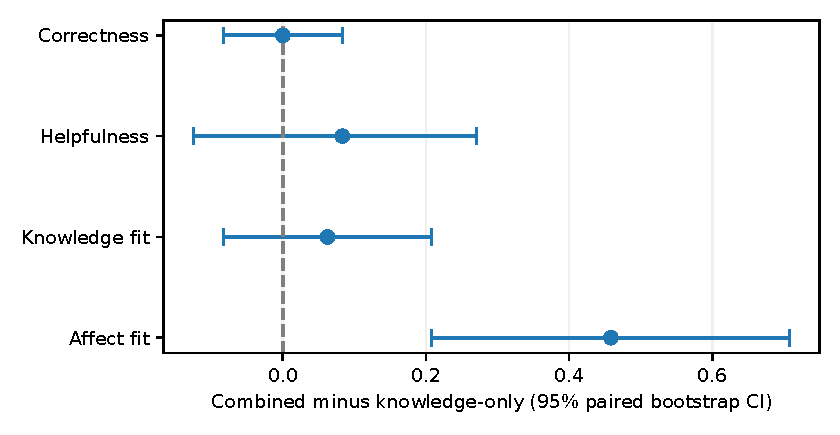
\includegraphics[width=\columnwidth]{phase5_paired_effects.pdf}\caption{Scenario-paired mean differences and 95\% bootstrap intervals.}\label{fig:effects}\end{figure}
\subsection{Cross-Phase Interpretation}
The RoBERTa gain in macro-F1 supports transformer-based text representation, but the final macro-F1 below 0.50 indicates remaining class-level errors. Reddit language cannot be assumed to represent classroom discourse. Phase IV therefore uses predicted affect as an illustrative conditioning signal, not a verified measurement of a learner's emotional state.

In Phase III, the improvement in AUC is supported by learner-cluster resampling and disappears under the shuffled-behavior control. The result suggests that temporal activity patterns contain information beyond knowledge-history variables. Nevertheless, attempts, timing, and similar behavioral proxies can also reflect task difficulty and platform usage. They should not be renamed emotional observations.

Phase IV's automated checks establish policy conformance, not pedagogical efficacy. Phase V addresses a different question by collecting human ratings. The combined condition improves affective appropriateness, but the other three criteria show no significant change after Holm correction. This pattern is consistent with affect-conditioned wording rather than a change in instructional decisions. The many zero paired differences also constrain sensitivity to small effects.

\subsection{Reproducibility and Reporting}
Reproduction requires preserving the GoEmotions single-label filter and held-out partition, performing learner-disjoint educational splitting before model fitting, and ensuring that feature windows use past events only. Each tutoring scenario must have one response for each of four policy variants. Evaluator workbooks should be joined on response IDs, and paired confidence intervals should resample scenarios rather than individual rubric scores. Independent provenance of evaluators and effectiveness in real learners remain separate validation requirements.

\section{Limitations and Threats to Validity}
\textit{Dataset alignment:} GoEmotions is Reddit-derived and does not measure the emotions of learners in the educational dataset. The two data sources have no common learner identifiers or synchronized observations. Consequently, no joint affect--knowledge model has been trained or evaluated on matched learners.

\textit{Response construction:} The scenarios were written by researchers, the knowledge probabilities were illustrative, and the tutoring outputs were fixed templates. A policy response can appear affectively suitable without changing actual student understanding. The 96 responses are nested within 24 scenarios, so scenario-paired inference is more appropriate than treating all ratings as independent observations.

\textit{Human evaluation:} The workbooks contain complete paired scores and distinct evaluator IDs; evaluator independence is reported by the authors and has not been externally audited. Ratings are subjective and restricted to three mathematics domains. No real student interaction, retention, achievement, or engagement was measured. Thus, the result should be described as improved \emph{rated affective appropriateness} rather than improved learning effectiveness.

\section{Conclusion}
AKC-Tutor demonstrates three reproducible component-level findings: transformer-based emotion recognition outperforms a sparse-text baseline on a single-label GoEmotions task; behavioral-history features add predictive value to educational knowledge features under learner-disjoint evaluation; and affect-conditioned templates improve human-rated affective appropriateness in controlled scenarios. The combined response policy did not significantly improve correctness, helpfulness, or knowledge fit relative to knowledge-only tutoring. Future work requires synchronized educational dialogue and learner histories, real learner studies, and outcome-based evaluation before claims of end-to-end affect-aware tutoring effectiveness can be made.

\begin{thebibliography}{99}
\bibitem{piech2015} C. Piech \emph{et al.}, ``Deep Knowledge Tracing,'' in \emph{NeurIPS}, 2015.
\bibitem{wang2024} S. Wang \emph{et al.}, ``Artificial intelligence in education: A systematic literature review,'' \emph{Expert Systems with Applications}, vol. 252, Art. 124167, 2024, doi: 10.1016/j.eswa.2024.124167.
\bibitem{demszky2020} D. Demszky \emph{et al.}, ``GoEmotions: A dataset of fine-grained emotions,'' in \emph{ACL}, 2020, doi: 10.18653/v1/2020.acl-main.372.
\bibitem{liu2019} Y. Liu \emph{et al.}, ``RoBERTa: A robustly optimized BERT pretraining approach,'' arXiv:1907.11692, 2019.
\bibitem{liebenow25} L. W. Liebenow et al., ``Self-assessment accuracy in the age of artificial intelligence: Differential effects of LLM-generated feedback,'' \emph{Computers and Education}, doi: 10.1016/j.compedu.2025.105385.
\bibitem{xu23} J. Xu et al., ``Improving knowledge tracing via a heterogeneous information network enhanced by student interactions,'' \emph{Expert Systems with Applications}, doi: 10.1016/j.eswa.2023.120853.
\bibitem{sun24} X. Sun et al., ``Target hierarchy-guided knowledge tracing: Fine-grained knowledge state modeling,'' \emph{Expert Systems with Applications}, doi: 10.1016/j.eswa.2024.123898.
\bibitem{zhao23} Y. Zhao et al., ``Exploiting multiple question factors for knowledge tracing,'' \emph{Expert Systems with Applications}, doi: 10.1016/j.eswa.2023.119786.
\bibitem{huang24speed} T. Huang et al., ``Response speed enhanced fine-grained knowledge tracing: A multi-task learning perspective,'' \emph{Expert Systems with Applications}, doi: 10.1016/j.eswa.2023.122107.
\bibitem{huang24causal} C. Huang et al., ``Learning consistent representations with temporal and causal enhancement for knowledge tracing,'' \emph{Expert Systems with Applications}, doi: 10.1016/j.eswa.2023.123128.
\bibitem{zhu24} M. Zhu, L. Qiu, and J. Zhou, ``Meta-path structured graph pre-training for improving knowledge tracing in intelligent tutoring,'' \emph{Expert Systems with Applications}, doi: 10.1016/j.eswa.2024.124451.
\bibitem{huang24moe} T. Huang et al., ``Pull together: Option-weighting-enhanced mixture-of-experts knowledge tracing,'' \emph{Expert Systems with Applications}, doi: 10.1016/j.eswa.2024.123419.
\bibitem{duan24} Z. Duan et al., ``Towards more accurate and interpretable model: Fusing multiple knowledge relations into deep knowledge tracing,'' \emph{Expert Systems with Applications}, doi: 10.1016/j.eswa.2023.122573.
\bibitem{liu24hyper} S. Liu et al., ``Hyperbolic embedding of discrete evolution graphs for intelligent tutoring systems,'' \emph{Expert Systems with Applications}, doi: 10.1016/j.eswa.2023.122451.
\bibitem{park24concept} S. Park et al., ``Enhancing knowledge tracing with concept map and response disentanglement,'' \emph{Knowledge-Based Systems}, doi: 10.1016/j.knosys.2024.112346.
\bibitem{yu25graph} G. Yu et al., ``Exploring long- and short-term knowledge state graph representations with adaptive fusion for knowledge tracing,'' \emph{Information Processing and Management}, doi: 10.1016/j.ipm.2025.104074.
\bibitem{sun24progress} J. Sun et al., ``Progressive knowledge tracing: Modeling learning process from abstract to concrete,'' \emph{Expert Systems with Applications}, doi: 10.1016/j.eswa.2023.122280.
\bibitem{yang24hetero} H. Yang et al., ``Heterogeneous graph-based knowledge tracing with spatiotemporal evolution,'' \emph{Expert Systems with Applications}, doi: 10.1016/j.eswa.2023.122249.
\bibitem{liu26contrast} J. Liu et al., ``Heterogeneous graph knowledge tracing with novel contrastive view and meta-path contexts,'' \emph{Expert Systems with Applications}, doi: 10.1016/j.eswa.2025.128840.
\bibitem{yang25mahkt} H. Yang et al., ``MAHKT: Knowledge tracing with multi-association heterogeneous graph embedding based on knowledge transfer,'' \emph{Knowledge-Based Systems}, doi: 10.1016/j.knosys.2025.112958.
\bibitem{xu26sqg} T. Xu et al., ``SQGKT: Student-question interaction graph-based knowledge tracing,'' \emph{Expert Systems with Applications}, doi: 10.1016/j.eswa.2025.129175.
\bibitem{luo24} H. Luo et al., ``An efficient state-aware coarse-fine-grained model for knowledge tracing,'' \emph{Knowledge-Based Systems}, doi: 10.1016/j.knosys.2024.112375.
\bibitem{wang25states} S. Wang et al., ``Learning states enhanced knowledge tracing: Simulating the diversity in real-world learning process,'' \emph{Expert Systems with Applications}, doi: 10.1016/j.eswa.2025.126838.
\bibitem{wu25cognitive} Q. Wu et al., ``Graph knowledge tracing in cognitive situation: Validation of classic assertions in cognitive psychology,'' \emph{Knowledge-Based Systems}, doi: 10.1016/j.knosys.2025.113281.
\bibitem{wu24program} Y. Wu et al., ``Programming knowledge tracing based on heterogeneous graph representation,'' \emph{Knowledge-Based Systems}, doi: 10.1016/j.knosys.2024.112161.
\bibitem{xiao26} X. Xiao et al., ``Information processing dynamic graph for knowledge tracing,'' \emph{Information Processing and Management}, doi: 10.1016/j.ipm.2025.104331.
\bibitem{yu24emotion} S. Yu et al., ``Bridging computer and education sciences: A systematic review of automated emotion recognition in online learning environments,'' \emph{Computers and Education}, doi: 10.1016/j.compedu.2024.105111.
\bibitem{affect26} ``Affective computing in online higher education: A systematic literature review,'' \emph{Computers and Education: Artificial Intelligence}, doi: 10.1016/j.caeai.2025.100499.
\bibitem{zhang24video} C. Zhang et al., ``Guiding student learning in video lectures: Effects of instructors' emotional expressions and visual cues,'' \emph{Computers and Education}, doi: 10.1016/j.compedu.2024.105062.
\end{thebibliography}
\end{document}
